\documentclass{scrartcl}

\usepackage[utf8]{inputenc}
\usepackage[T1]{fontenc}
\usepackage{lmodern}
\usepackage[ngerman]{babel}
\usepackage{amsmath}
\usepackage{listings}
\usepackage{graphicx}
\usepackage{float}

\usepackage{color} 

%% Commands
\newcommand{\n}{\newline}

\title{User Manual}
\subtitle{King of Jawa}
\author{Pascal Bürklin, Isabel Geissmann, Jannik Jaberg, Nikolai Rutz}
\date{\today}
\begin{document}
\maketitle
\begin{figure}[H]
	
\includegraphics[width=\linewidth]{LOGO.png}
\end{figure}
\tableofcontents
\pagebreak
\section{Starten von King of Jawa}

Um das Spiel zu Starten muss als erstes ein Server gestartet werden. Dies erfolgt über die Kommandozeile (Das Kommandofenster muss im Ordner gestartet werden in dem sich die .jar Datei befindet).
\begin{center}
    java -jar “King of Java-0.0.1.jar” server <port>
\end{center}
Angewandt sieht dies so aus:
\begin{center}
    java -jar “King of Java-0.0.1.jar” server 22313
\end{center}
\begin{figure}[H]
	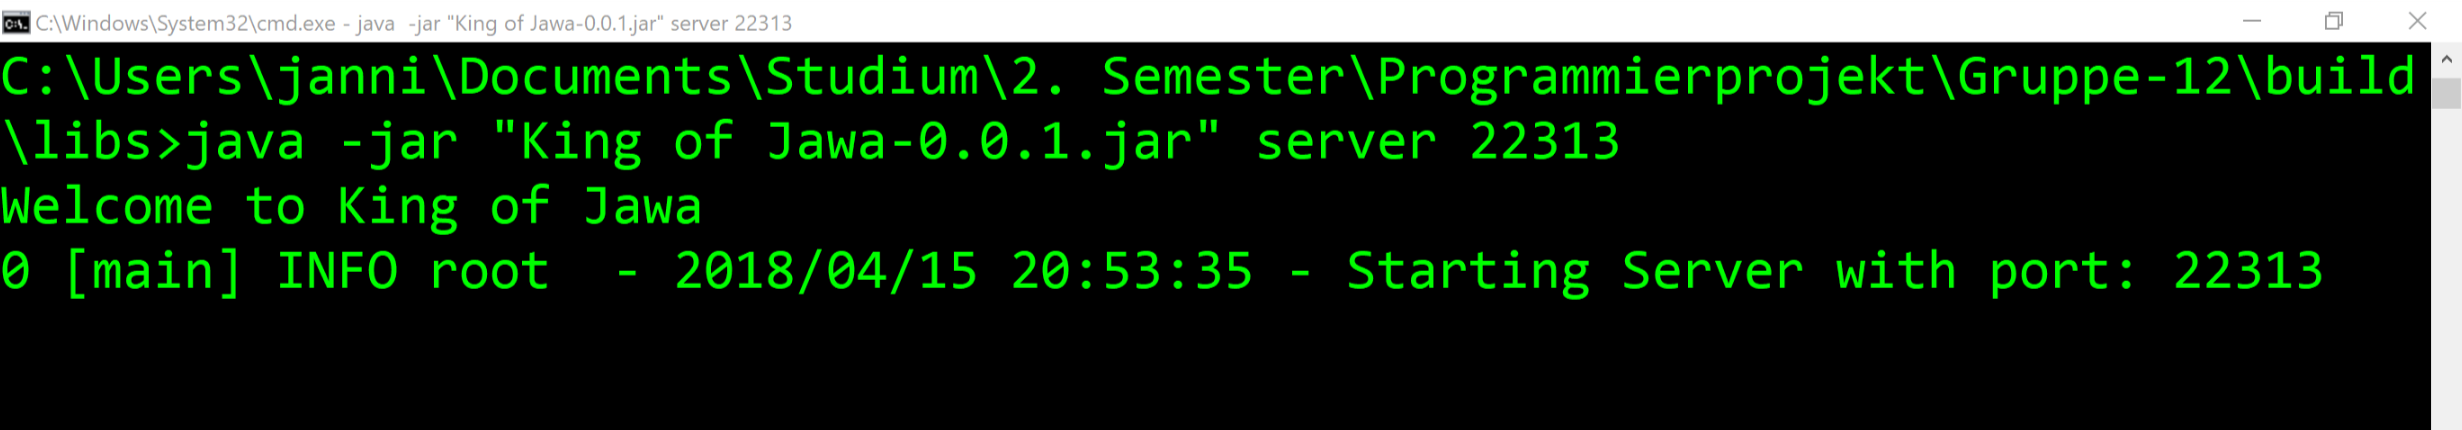
\includegraphics[width=\linewidth]{CMDserver.png}
	\caption{Konsolen-Output Server}
	\label{fig:map1}
\end{figure}
Danach kann das Spiel mit folgendem Befehl gestartet werden:
\begin{center}
    java -jar “King of Java-0.0.1.jar” client <host>:<port> $[<username>]$ 
\end{center}
Wobei der Username fakultativ ist. Ist kein Username angegeben so wird automatisch der Systemname verwendet. Der Name kann während dem Spiel jederzeit mit dem Command /nick oder über den Button geändert werden.\n
Bei dem Host handelt es sich um die IPv4 Adresse des Computers auf dem der Server gestartet wurde. \n
Angewandt sieht dies so aus:
\begin{center}
    java -jar “King of Java-0.0.1.jar” client 192.168.1.122:22313 XxXLaNlOrDXxX
\end{center}
\begin{figure}[H]
	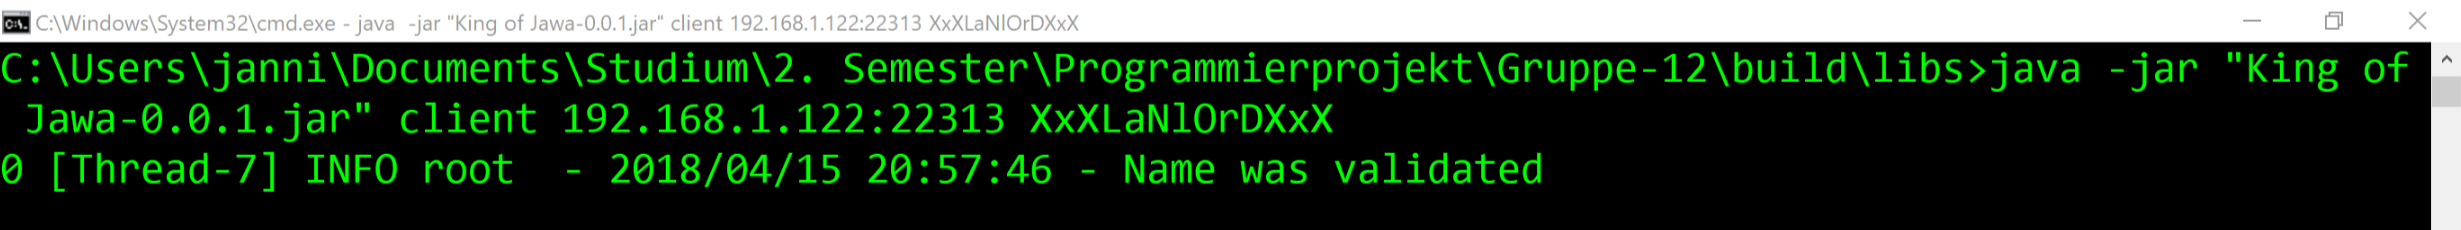
\includegraphics[width=\linewidth]{CMDclient.png}
	\caption{Konsolen-Output Client}
	\label{fig:map1}
\end{figure}
\pagebreak
Wenn alles richtig eingegeben wurde öffnet sich das Spiel. Sobald das Intro fertig ist muss die Leertaste gedrückt werden um ins Hauptmenu zu gelangen.
\begin{figure}[H]
	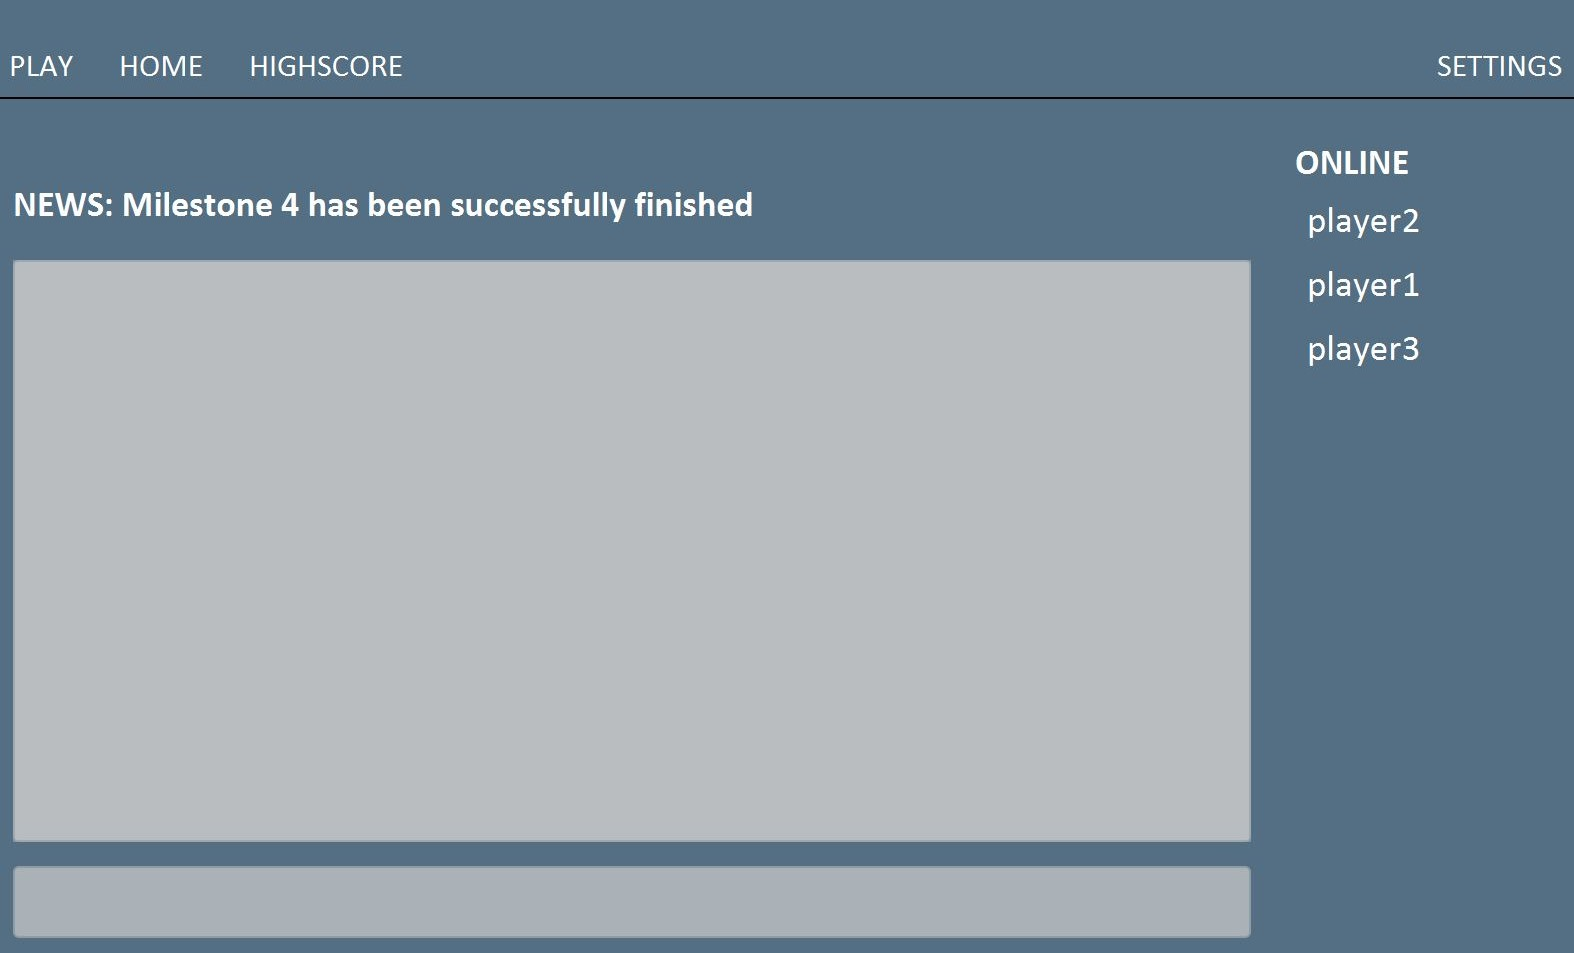
\includegraphics[width=\linewidth]{HomeScreen.JPG}
	\caption{Home-Screen}
	\label{fig:HomeScreen}
\end{figure} 
Im Hauptmenu befindet sich der Global-Chat und es wird auf der rechten Seite eine Liste mit allen Spielern angezeigt. In der ersten Zeile befinden sich alle Knöpfe. Um ein Spiel zu beginnen bzw. um eine Lobby zu erstellen, muss der Spieler/die Spielerin auf den ersten Knopf drücken. Mit dem Home-Knopf ist es möglich, jederzeit in diesen Home-Screen zurückzukehren.
Mit einem Klick auf den Highscore-Knopf öffnet sich dieser und die besten Player werden angezeigt. An erster Stelle im Highscore steht, wer am meisten Punkte pro Minute erzielt hat.


\begin{figure}[H]
	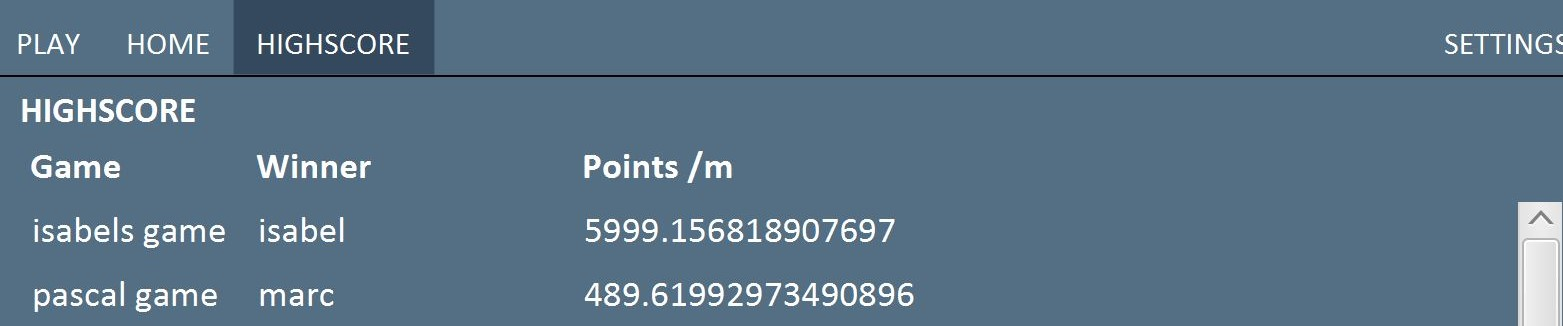
\includegraphics[width=\linewidth]{highscore.JPG}
	\caption{Highscore}
	\label{fig:Highscore}
\end{figure}


\pagebreak
\section{Commands}
\begin{itemize}
    \item /nick <newname>
    \item /whisper <\grqq receipant\grqq> <message>
    \item /ping
	\item /g
	
\end{itemize}
\begin{center}
    \begin{tabular}{| p{6cm} | p{6cm} |}
        \hline
        \textbf{Anwendung} & \textbf{Nutzen} \\ \hline
        /nick Maximumblyat & ändert deinen Namen   \\ \hline
        /whisper "Habibi" \space GiT GuD & sendet die Nachricht "Git GuD"\space an Habibi  \\ \hline
        /ping & gibt dir deinen Ping an  \\ \hline
        /g & wenn ihr in einer Lobby oder inGame seid, kann mit /g in den Global-Chat geschrieben werden. \\ \hline
    \end{tabular}
\end{center}
\begin{figure}[H]
	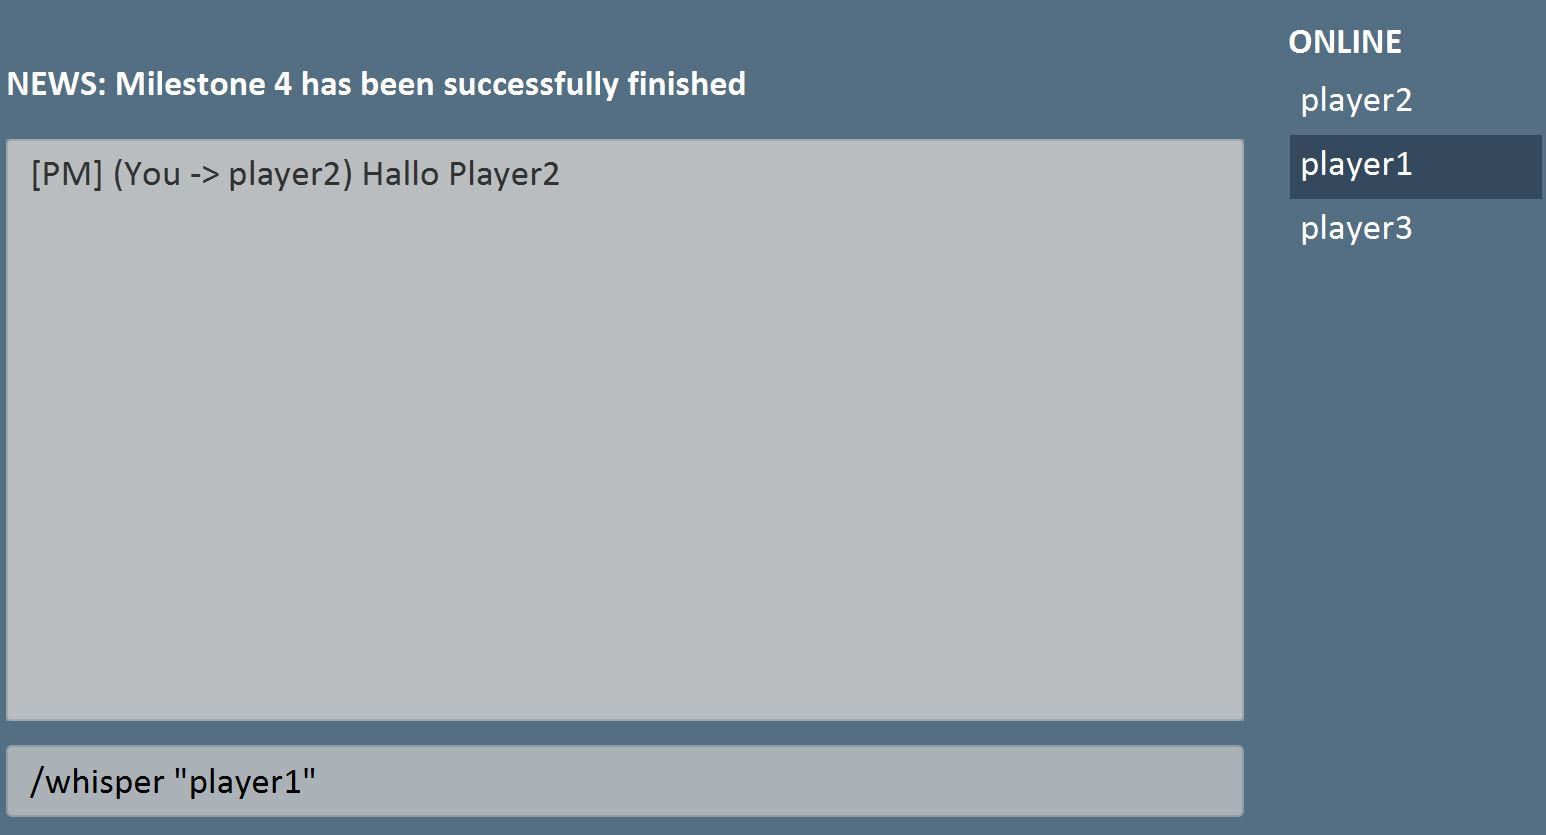
\includegraphics[width=\linewidth]{whisper2.JPG}
	\caption{Beispiel Commands: whisper}
	\label{fig:whisper}
\end{figure}
In der Tabelle sind alle Kommandos die wir in das Spiel eingefügt haben aufgelistet. Alle funktionieren nach dem gleichen Prinzip wie das whisper Kommando. Natürlich ist es auch möglich jemandem eine private Nachricht zu senden, ohne dass das Kommando von Hand eingetippt werden muss. Einfach ein Doppelklick auf den Spieler und schon kann die private Nachricht eingetippt werden.
\begin{figure}[H]
	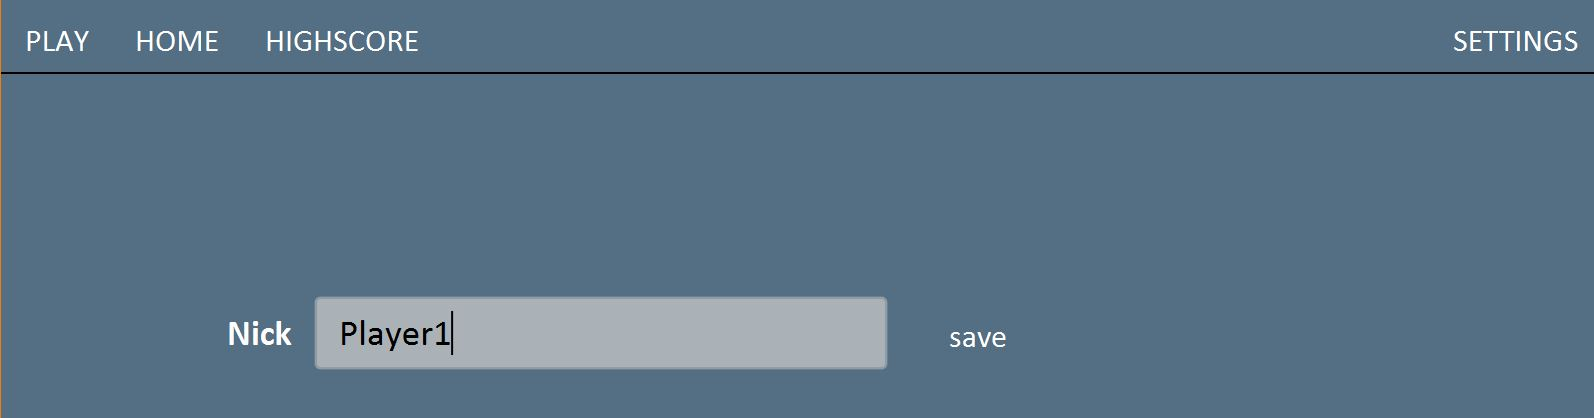
\includegraphics[width=\linewidth]{settings.JPG}
	\caption{Spielername ändern}
	\label{fig:chaningName}
\end{figure}
Nachdem der Settings-Knopf gedrückt wurde ist es möglich einen neuen Spielernamen zu wählen und diesen zu speichern. //
\subsection{Tastenfunktionen}
\begin{center}
    \begin{tabular}{| p{6cm} | p{6cm} |}
        \hline
        \textbf{Tasten} & \textbf{Nutzen} \\ \hline
        alt Enter & starten und beenden des Vollbildmodus   \\ \hline
		Pfeiltasten & bewegen auf der Karte im Spiel\\ 
		\hline
       	- & Bildausschnitt im Spiel vergrössern (rauszoomen)\\ \hline
    	+ & Bildausschnitt im Spiel verkleinern (reinzoomen)\\ \hline
    \end{tabular}
\end{center}

\pagebreak

\section{Lobby}
Um \textbf{King of Jawa} spielen zu können muss eine Lobby erstellt werden. Nachdem Play gedrückt wird, wechselt der untere Teil des Fensters. Mit dem Create-Knopf untern rechts kann eine neue Lobby erstellt werden. Sobald eine Lobby erstellt wurde können die anderen Spieler dieser mit einem Doppelklick beitreten.
\begin{figure}[H]
	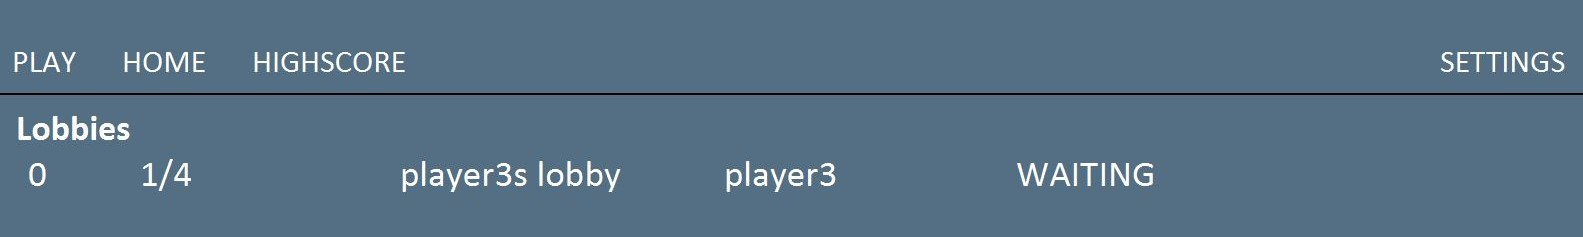
\includegraphics[width=\linewidth]{joiningLobby.JPG}
	\caption{Lobby joining}
	\label{fig:joiningLobby}
\end{figure}
Die wartenden Spieler können sich im Lobby-Chat unterhalten. Sobald alle Spieler, in einer Lobby, den Ready-Knopf gedrückt haben, kann der Lobby owner das Spiel starten. 
\begin{figure}[H]
	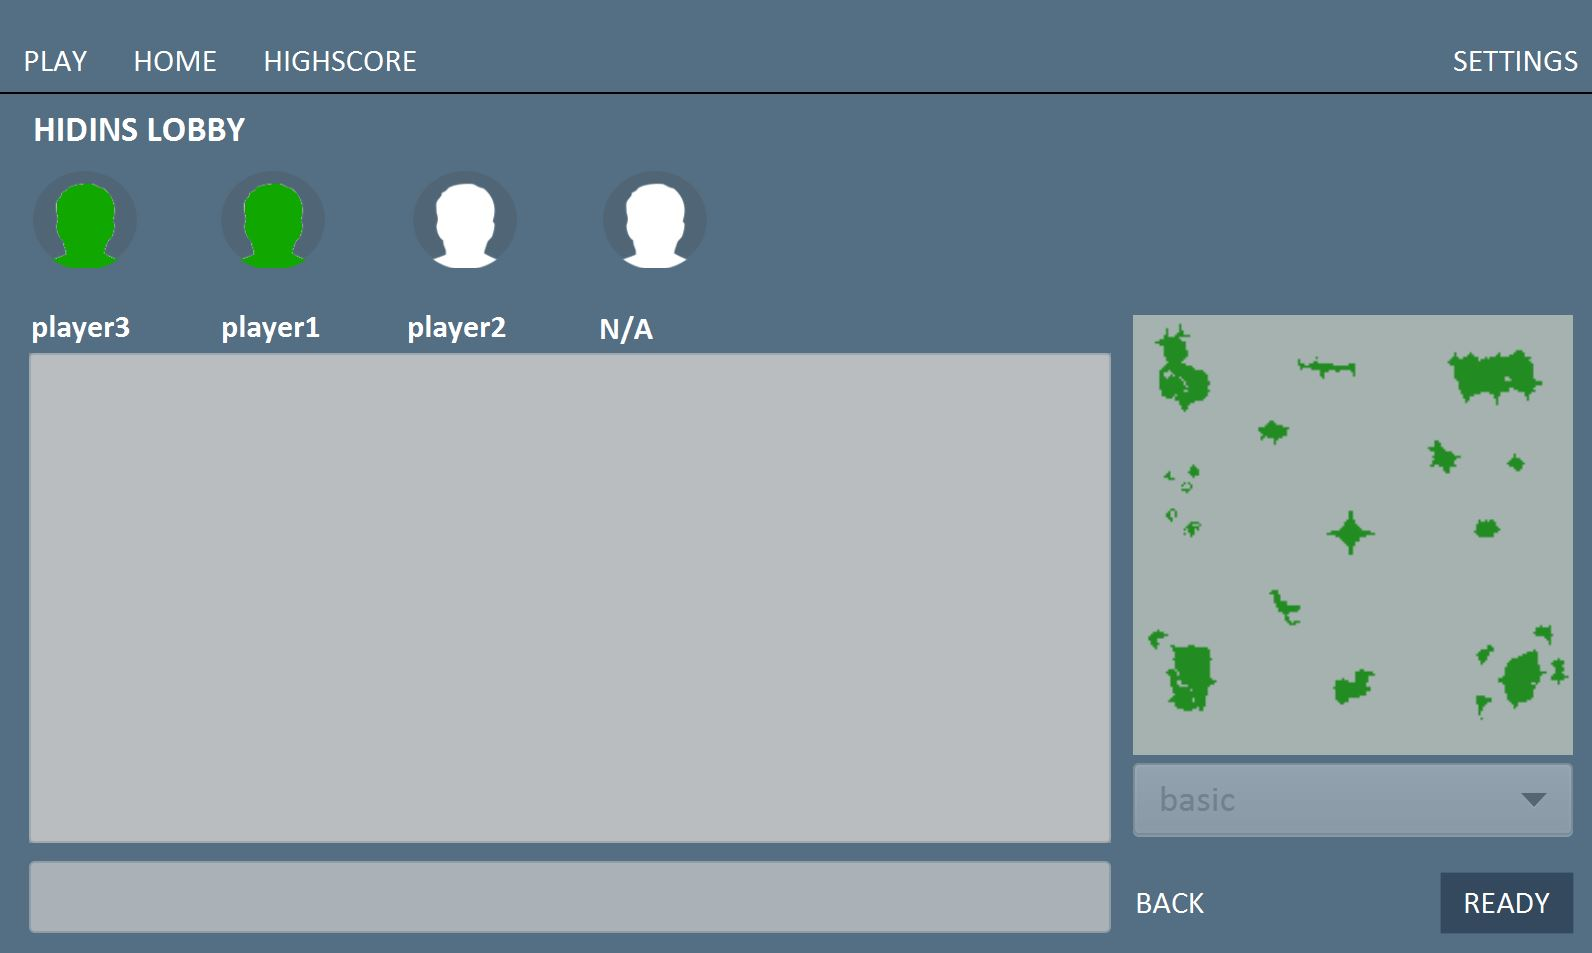
\includegraphics[width=\linewidth]{readylobby.JPG}
	\caption{Lobby ready}
	\label{fig:readyLobby}
\end{figure}

\pagebreak
\section{Spielregeln}
Direkt nach Spielstart muss sich jeder Spieler/jede Spielerin für eine Insel entscheiden und dort die Base bauen. Danach gehört diese Insel euch und ihr könnt beginnen eure Metropole aufzubauen.

\begin{figure}[H]
	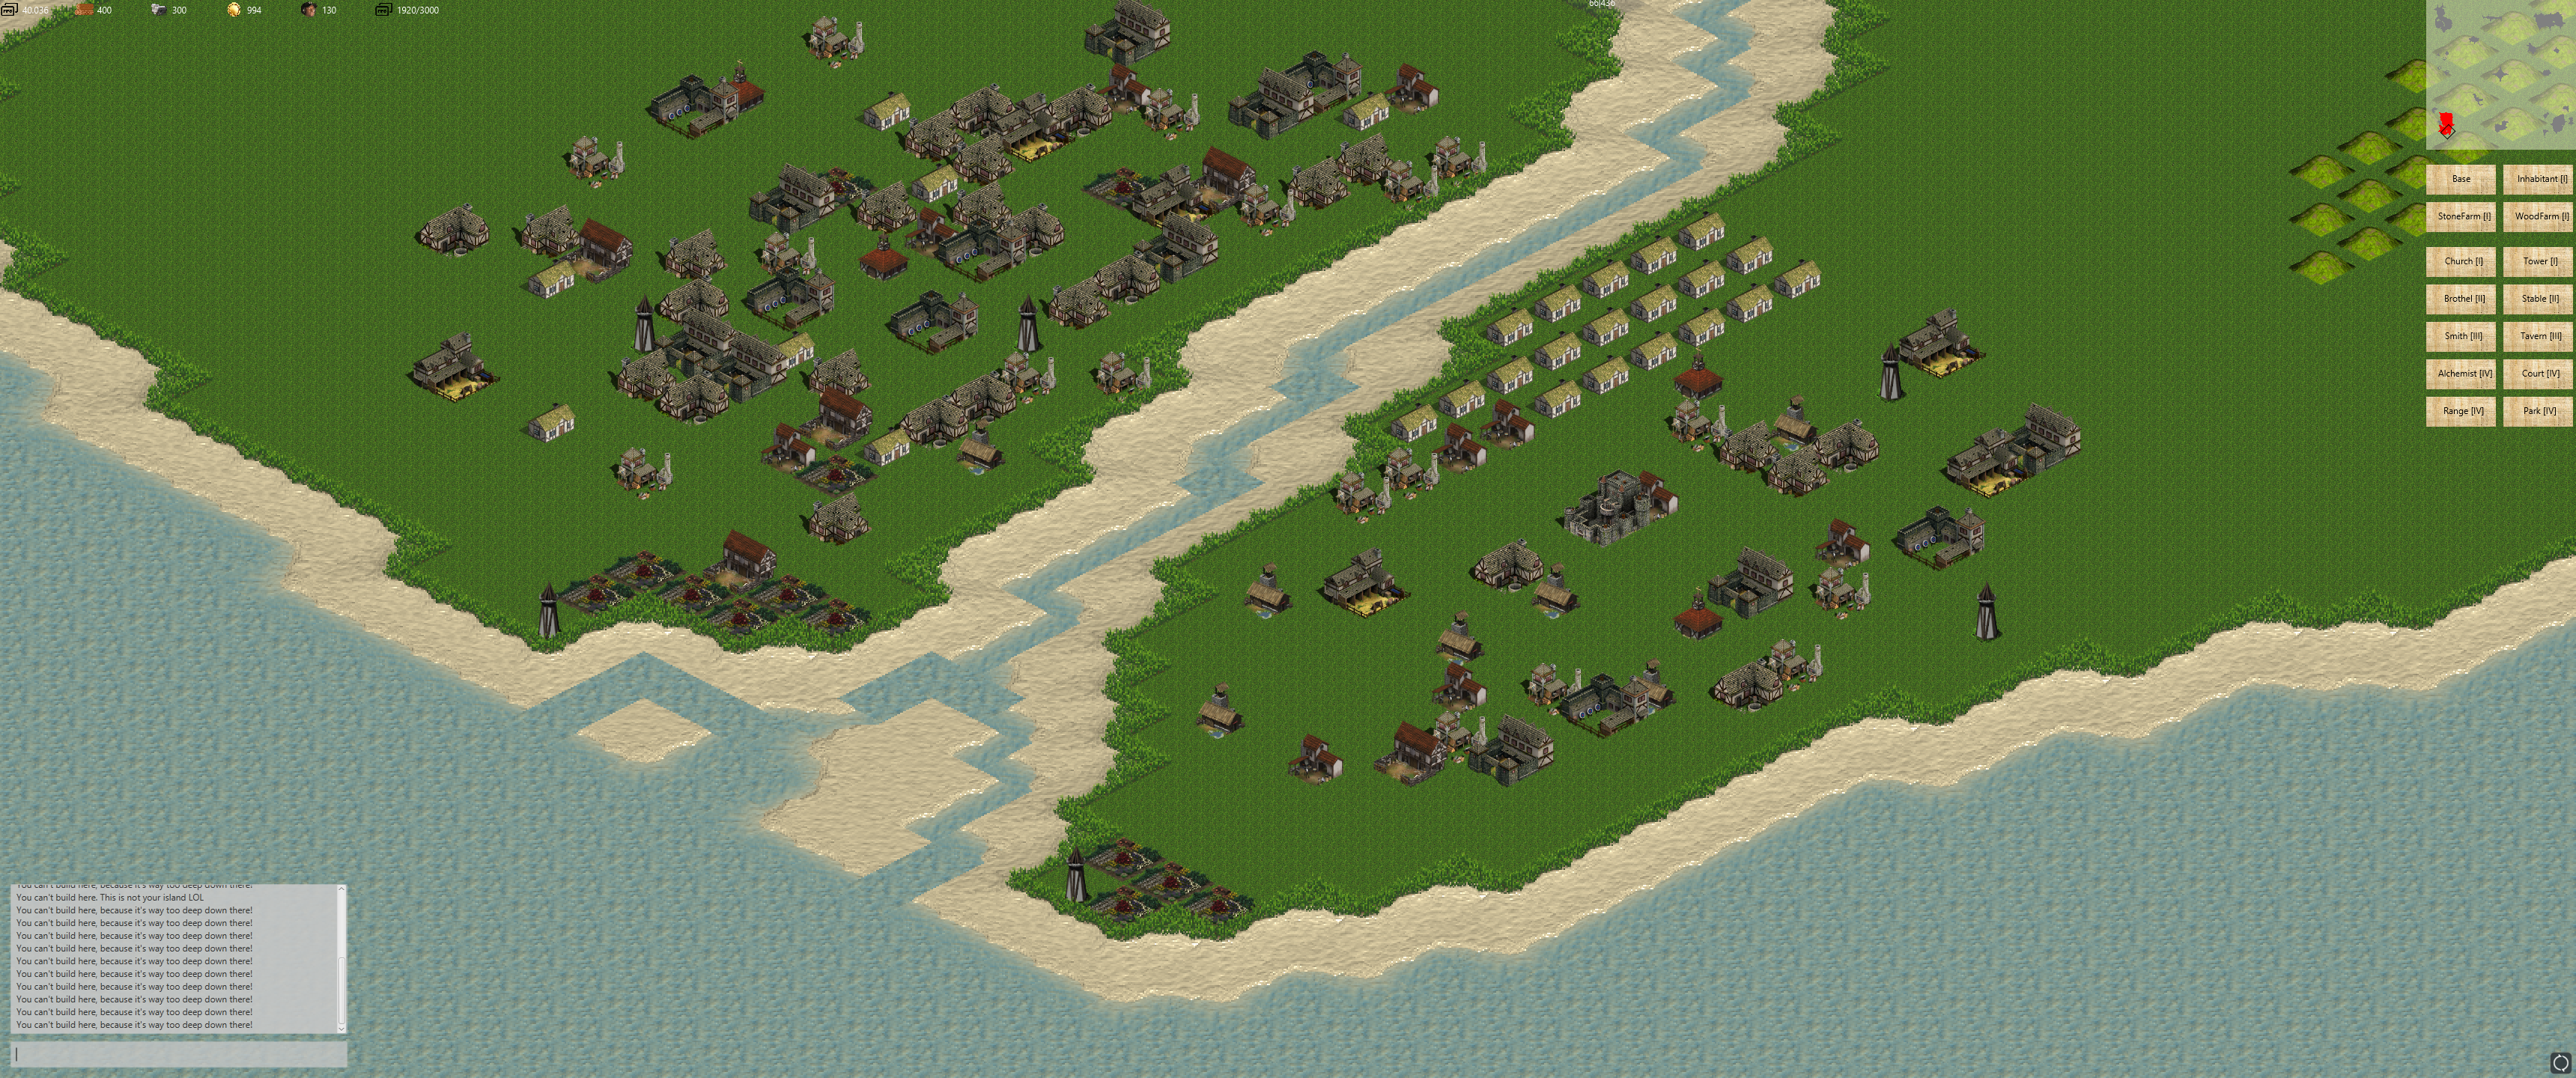
\includegraphics[width=\linewidth]{kingofjawa.png}
	\caption{King of Jawa}
	\label{fig:kingofjawa}
\end{figure}

\subsection{Ressourcen}
Es gibt drei verschiedene Typen von Ressourcen Holz, Stein und Gold. Oben links im Fenster sieht man wie viel Einheiten pro Ressource vorhanden sind. 
\subsection{Mini-Map}
Oben rechts im Fenster seht ihr eine Mini-Map bei der in Farbe markiert ist, ob eine Insel frei oder vergeben ist. Mittels klick auf die Mini-Map könnt ihr zum ausgewählten Punkt springen.
\subsection{Gebäude}
Unterhalb der Mini-Map befinden sich die Buttons um die verschiedenen Gebäude zu bauen. Bei den oberen vier Buttons handelt es sich um die Base und die Ressourcen Gebäude und bei den anderen um die Spass-Gebäude. Neben dem Namen der Gebäude steht ab welchem Level diese verfügbar sind.
An dieser Stelle soll noch nicht zu viel verraten werden. Teil des Spiel ist es herauszufinden was die beste Strategie ist um den Metropolen-Status zu erreichen. 
\subsubsection{Base}
\begin{minipage}{0.3\textwidth}
	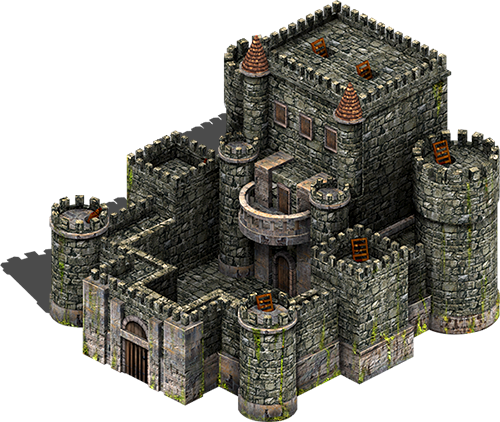
\includegraphics[width=\textwidth]{imgBase.png}
\end{minipage}
\hfill
\begin{minipage}{0.5\textwidth}
	\textbf{Base} \\
	Sobald die Base auf einer Insel gebaut wurde hat man diese eingenommen und kann weitere Gebäude bauen.\\

	Die Base hat 5 verschiedene Levels. Mit einem Rechtsklick auf die Base kann überprüft werden in welchem Level die Base ist und wie viel ein Level-up kostet.\\
	
\end{minipage}

\subsubsection{Resourcen-Gebäude}
Die Ressourcen-Gebäude liefern dem Spieler/der Spielerin neue Ressourcen. Je nachdem in welchem der sieben Levels das Gebäude ist, bringt es mehr oder weniger Ressourcen. Mit einem Rechtsklick auf das Gebäude ist ersichtlich wie viel ein Level-up kostet.\n
\n

\begin{minipage}{0.3\textwidth}
	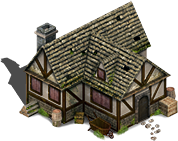
\includegraphics[width=\textwidth]{imgWoodFarm.png}
\end{minipage}
\hfill
\begin{minipage}{0.5\textwidth}
	\textbf{Holz-Farm}\\
	Die Holz-Farm liefert dem Spieler/der Spielerin neue Holz und Gold Ressourcen.\\
\end{minipage}

\begin{minipage}{0.3\textwidth}
	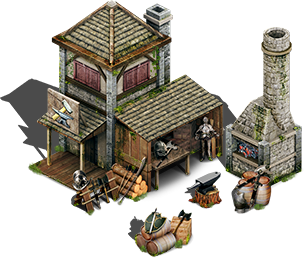
\includegraphics[width=\textwidth]{imgStoneFarm.png}
\end{minipage}
\hfill
\begin{minipage}{0.5\textwidth}
	\textbf{Stein-Farm}\\
	Die Stein-Farm liefert dem Spieler/der Spielerin neue Stein und Gold Ressourcen.\\

\end{minipage}

\begin{minipage}{0.3\textwidth}
	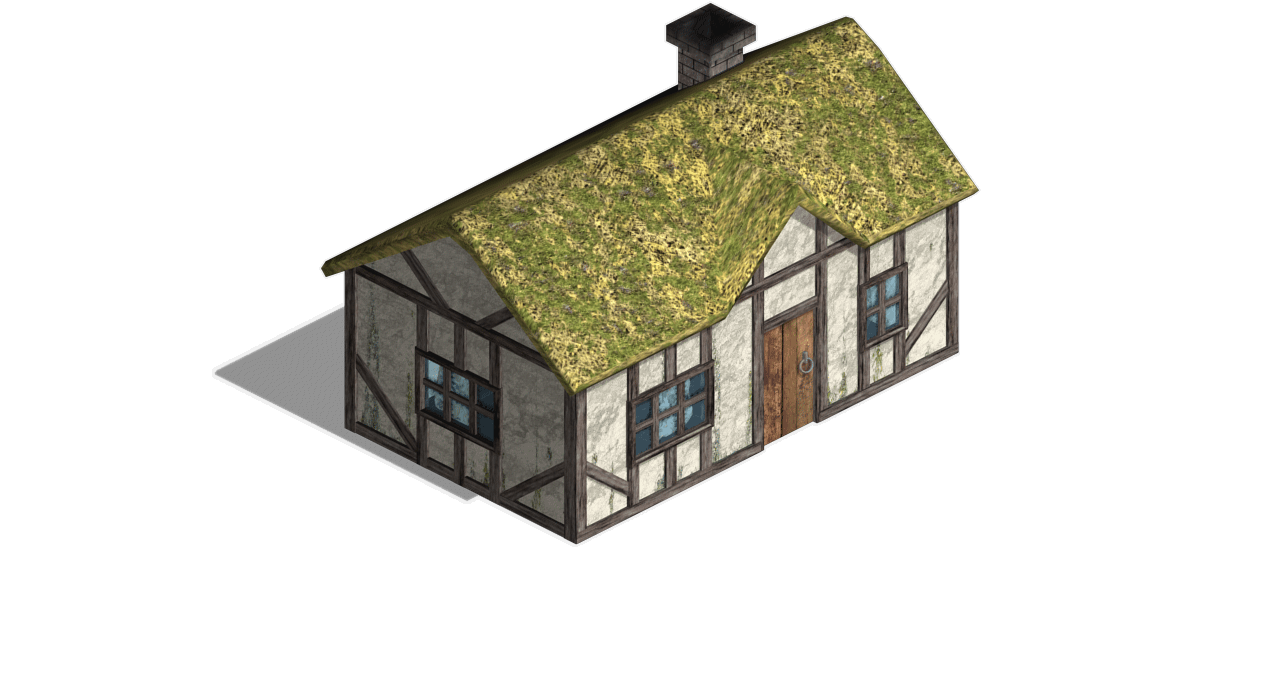
\includegraphics[width=\textwidth]{imgInhabitant.png}
\end{minipage}
\hfill
\begin{minipage}{0.5\textwidth}
	\textbf{Einwohner-Haus}\\
	Das Einwohner-Haus liefert dem Spieler/der Spielerin neue Gold Ressourcen.\\

\end{minipage}

\subsubsection{Spass-Gebäude}
Die Spass-Gebäude haben nur einen Level. Je nachdem in welchem Level die Base ist sind unterschiedliche Gebäude verfügbar. Die Gebäuse kosten unterschiedlich viel und liefern unterschiedliche Faktoren damit die Ressourcen schneller anwachsen.\n
\n
\begin{minipage}{0.3\textwidth}
	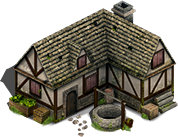
\includegraphics[width=\textwidth]{imgAlchemist.png}
\end{minipage}
\hfill
\begin{minipage}{0.5\textwidth}
	\textbf{Alchemist}\\

	\textbf{Verfügbar ab: }\\ Base Level 4\\
	\textbf{Kosten:
	}\\
	Gold: 1800 \\
	Holz: 900\\
	
\end{minipage}

\begin{minipage}{0.3\textwidth}
	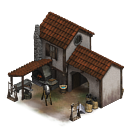
\includegraphics[width=\textwidth]{imgBrothel.png}
\end{minipage}
\hfill
\begin{minipage}{0.5\textwidth}
	\textbf{Freudenhaus}\\
	
	\textbf{Verfügbar ab: }\\ Base Level 2\\
	\textbf{Kosten:
	}\\
	Gold: 700 \\
	Holz: 150\\
	
\end{minipage}

\begin{minipage}{0.3\textwidth}
	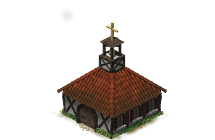
\includegraphics[width=\textwidth]{imgChurch.png}
\end{minipage}
\hfill
\begin{minipage}{0.5\textwidth}
	\textbf{Kirche} 
	
	\textbf{Verfügbar ab: }\\ Base Level 1\\
	\textbf{Kosten:
	}\\
	Gold: 250 \\
	Holz: 100\\
	Stein: 50\\
	
\end{minipage}

\begin{minipage}{0.3\textwidth}
	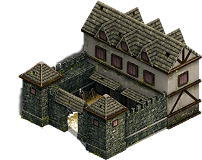
\includegraphics[width=\textwidth]{imgCourt.png}
\end{minipage}
\hfill
\begin{minipage}{0.5\textwidth}
	\textbf{Gericht}\\
	
	\textbf{Verfügbar ab: }\\ Base Level 4\\
	\textbf{Kosten:
	}\\
	Gold: 2200 \\
	Stein: 500\\
	
\end{minipage}

\begin{minipage}{0.3\textwidth}
	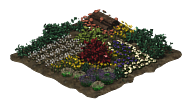
\includegraphics[width=\textwidth]{imgPark.png}
\end{minipage}
\hfill
\begin{minipage}{0.5\textwidth}
	\textbf{Park}\\
	
	\textbf{Verfügbar ab: }\\ Base Level 4\\
	\textbf{Kosten:
	}\\
	Holz: 1200\\
	Stein: 600\\
	
\end{minipage}

\begin{minipage}{0.3\textwidth}
	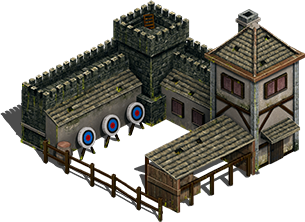
\includegraphics[width=\textwidth]{imgRange.png}
\end{minipage}
\hfill
\begin{minipage}{0.5\textwidth}
	\textbf{Range}\\
	
	\textbf{Verfügbar ab: }\\ Base Level 4\\
	\textbf{Kosten:
	}\\
	Gold: 1200 \\
	Holz: 1200\\
	Stein: 800\\
	
\end{minipage}

\begin{minipage}{0.3\textwidth}
	
\includegraphics[width=\textwidth]{imgSmallTower.png}
\end{minipage}
\hfill
\begin{minipage}{0.5\textwidth}
	\textbf{Turm}\\

	\textbf{Verfügbar ab: }\\ Base Level 1\\
	\textbf{Kosten:
	}\\
	Gold: 100 \\
	Holz: 50\\
	
\end{minipage}

\begin{minipage}{0.3\textwidth}
	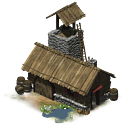
\includegraphics[width=\textwidth]{imgSmith.png}
\end{minipage}
\hfill
\begin{minipage}{0.5\textwidth}
	\textbf{Schmied}\\
	
	\textbf{Verfügbar ab: }\\ Base Level 3\\
	\textbf{Kosten:
	}\\
	Gold: 100 \\
	Holz: 50\\
	
\end{minipage}

\begin{minipage}{0.3\textwidth}
	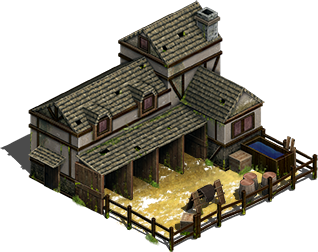
\includegraphics[width=\textwidth]{imgStable.png}
\end{minipage}
\hfill
\begin{minipage}{0.5\textwidth}
	\textbf{Stall}\\
	
	\textbf{Verfügbar ab: }\\ Base Level 2\\
	\textbf{Kosten:
	}\\
	Gold: 200 \\
	Holz: 300\\
	Stein: 100\\
	
\end{minipage}

\begin{minipage}{0.3\textwidth}
	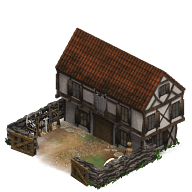
\includegraphics[width=\textwidth]{imgTavern.png}
\end{minipage}
\hfill
\begin{minipage}{0.5\textwidth}
	\textbf{Tavern}\\
	
	\textbf{Verfügbar ab: }\\ Base Level 3\\
	\textbf{Kosten:
	}\\
	Gold: 1200 \\
	Holz: 500\\
	Stein: 200\\
	
\end{minipage}
\end{document}